\section{Introduction}

\begin{frame}
  \frametitle{High Performance Computing}
  \begin{columns}
    \column{.5\textwidth}
    \begin{center}
      \begin{figure}
        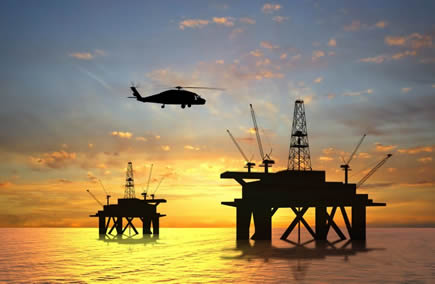
\includegraphics[scale=0.2]{figs/oil-gas-industry.jpg}\\
      \end{figure}
      \vspace{0.5cm}
      Oil and Gas
      \begin{figure}
        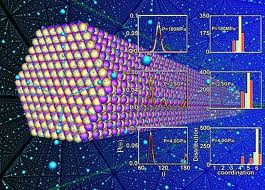
\includegraphics[scale=0.3]{figs/scientific-computing.jpg}\\
      \end{figure}
      Scientific Computing
    \end{center}
    \column{.5\textwidth}
    \begin{center}
      \begin{figure}
        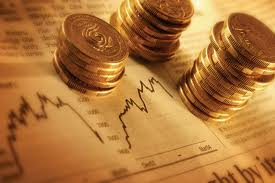
\includegraphics[scale=0.31]{figs/finance.jpg}\\
      \end{figure}
      \vspace{0.5cm}
      Finance
      \begin{figure}
        
\includegraphics[scale=0.31]{figs/ads.jpg}\\
      \end{figure}
      Online Advertising
    \end{center}
  \end{columns}
\end{frame}

\begin{frame}
  \frametitle{High Performance Computing}
  \begin{columns}
    \begin{column}{.5\textwidth}
      \begin{center}
        \begin{figure}
          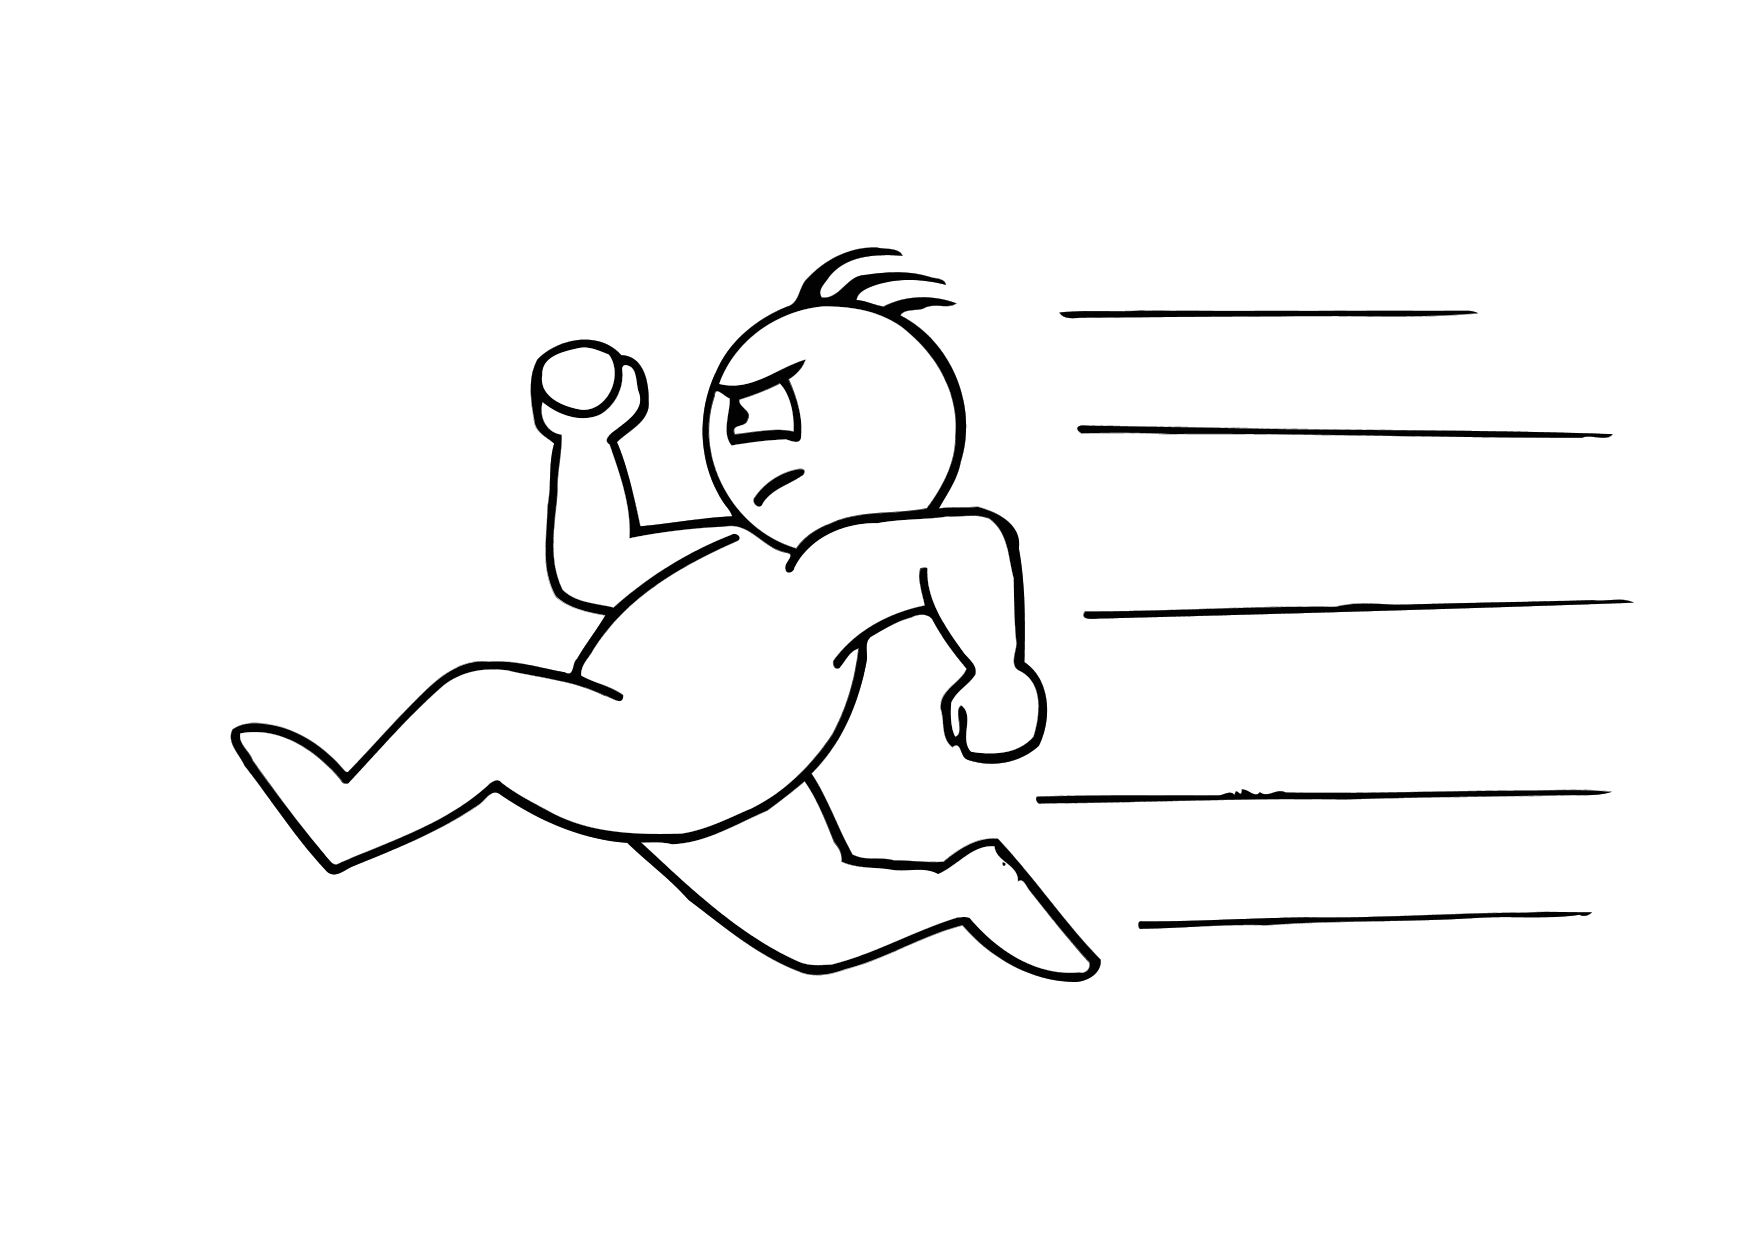
\includegraphics[scale=0.1, clip=true, trim=0 200 50 250]{figs/fast.jpg}\\
        \end{figure}
        Fast
      \end{center}
    \end{column}
    \begin{column}{.5\textwidth}
      \begin{center}
        \begin{figure}[!ht]
          \def\svgwidth{0.6\linewidth}
          \input{figs/energy-efficiency.pdf_tex}
        \end{figure}
        Energy Efficient
      \end{center}
    \end{column}
  \end{columns}
  \begin{center}
    \begin{figure}
      
\includegraphics[scale=0.3]{figs/productive.jpg}\\
    \end{figure}
    Productive
  \end{center}

\end{frame}

\begin{frame}{This Project}
  \begin{beamerboxesrounded}{Objectives}
    \begin{itemize}
    \item more efficient HPC -- using dataflow computing
    \item more productive HPC -- using aspect-oriented design
    \end{itemize}
  \end{beamerboxesrounded}
  \vspace{0.5cm}
  \begin{beamerboxesrounded}{Impact}
    \begin{itemize}
      \item first aspect-oriented compilation flow:
      \begin{itemize}
      \item for high-performance dataflow computing
      \item supporting run-time reconfiguration
      \end{itemize}
    \item 40--80\% code reduction, minimal performance overhead
    \item techniques deployed in FP7 HARNESS project
    \item best paper award candidate at ASAP 2013
    \end{itemize}
  \end{beamerboxesrounded}
\end{frame}

\begin{frame}
  \frametitle{Dataflow High-Performance Computing}
  \begin{figure}[!ht]
    \centering
    \def\svgwidth{0.9\linewidth}
    \input{figs/dataflow-both.pdf_tex}
  \end{figure}
\end{frame}

\begin{frame}
  \frametitle{CPU vs Dataflow}
  \begin{columns}
    \begin{column}{.5\linewidth}
      \begin{figure}[!ht]
        \centering
        \def\svgwidth{\linewidth}
        \input{figs/compute-cpu.pdf_tex}
      \end{figure}
      \begin{itemize}
      \item Fast to develop
      \item Inefficient
      \end{itemize}
    \end{column}
    \begin{column}{.5\linewidth}
      \begin{figure}[!ht]
        \centering
        \def\svgwidth{\linewidth}
        \input{figs/compute-dfe.pdf_tex}
      \end{figure}
      \begin{itemize}
      \item Slow to develop
      \item Efficient
      \end{itemize}
    \end{column}
  \end{columns}
\end{frame}

\begin{frame}[fragile]
  \frametitle{Kernel Optimisations: Bit Width}
  \begin{figure}[!ht]
    \centering
    \def\svgwidth{.7\linewidth}
    \input{figs/dfg-cast.pdf_tex}
  \end{figure}
\end{frame}

\begin{frame}[fragile]
  \frametitle{Kernel Optimisations: Stream Pipelineing}
  \begin{figure}[!ht]
    \centering
    \def\svgwidth{.7\linewidth}
    \input{figs/dfg-pipeline.pdf_tex}
  \end{figure}
\end{frame}

\begin{frame}[fragile]
  \frametitle{Kernel Optimisations: Pipeline Replication}
  \begin{figure}[!ht]
    \centering
    \def\svgwidth{.7\linewidth}
    \input{figs/dfg-parallel.pdf_tex}
  \end{figure}
\end{frame}

\begin{frame}[fragile]
  \frametitle{A Typical Dataflow Kernel: RTM}
  \begin{itemize}
  \item RTM - Reverse Time Migration for seismic imaging
  \item MaxJ - Java API for dataflow programming with FPGAs
  \end{itemize}

  \begin{lstlisting}
    // I/O type
    burstIn = new KArrayType(hwFloat(8,24), Par);

    // Compute type
    for (int i = 0; i < Par; i++)
      source[i] = burstIn[i].cast(hwFloat(8, 22));

    // Optimisations
    optimization.pushDSPFactor(1);

    // Pipeline replication
    for (int i = 0; i < Par; i++)
      result[i][0] = cur[0][6+i][5][5] * 2.0 - (...)
  \end{lstlisting}
\end{frame}

\begin{frame}[fragile]
  \frametitle{Issues}
  Developers must manually transform the original design to:
  \begin{enumerate}
  \item specify I/O type and width to interface with host API
  \item minimise compute type width to optimise resource usage
  \item specify casting between types to ensure correct values
  \item apply FPGA specific optimisations
  \item apply per stream or per block optimisation function calls
  \end{enumerate}

\end{frame}

\begin{frame}[fragile]
  \frametitle{Issues}
  \begin{beamerboxesrounded}{The Problem}
    Mixing optimisations with functional application code:
    \begin{itemize}
    \item harder to infer
    \item harder to automate
    \item less portable (cannot apply to other applications)
    \end{itemize}
  \end{beamerboxesrounded}
  \begin{beamerboxesrounded}{Our Solution}
    Decouple optimisations from application code:
    \begin{itemize}
    \item infer information as much as possible
    \item encapsulate optimisations in separate modules
    \item apply them automatically to explore the design space
    \end{itemize}
  \end{beamerboxesrounded}
\end{frame}
